% defining a if(plastex) environment
\newif\ifplastex
\plastexfalse

% defining a if(isinprint) environment
\newif\ifinprint
\ifdefined\isinprint
\inprinttrue
\else
\inprintfalse
\fi

% for the print, we use an extra b&w directory
\ifinprint
\newcommand{\rodinimgdir}{img-print}
\else
\newcommand{\rodinimgdir}{img}
\fi

\ifinprint
\def\doculist#1#2{
\begin{quote}
\hspace{-10mm}
\includegraphics[height=4ex]{#2}
\vspace{-8mm}

#1
\end{quote}
}
\else
\def\doculist#1#2{
\begin{quote}
\hspace{-10mm}
\textrm{\includegraphics[width=7mm]{#2}} % Hack!  We "mark" the image with textrm so that we can use a different CSS-Style in plastex.
\vspace{-8mm}

#1
\end{quote}
}
\fi

% dimensions on the title page
\newlength{\titletop}
\newlength{\titlesubtitledistance}
\newlength{\titlebottom}
\newlength{\titlesecdistance}
\ifinprint
\def\titledimrodin{\fontsize{30}{50}}
\def\titledimhandbook{\fontsize{20.5}{25}}
\def\titledimsubtext{\fontsize{13}{16}}
\def\titledimsponsor{\fontsize{11}{15}}
\setlength{\titletop}{120mm}
\setlength{\titlesubtitledistance}{2mm}
\setlength{\titlebottom}{-30mm}
\setlength{\titlesecdistance}{8mm}
\else
\def\titledimrodin{\fontsize{40}{50}}
\def\titledimhandbook{\fontsize{24.5}{30}}
\def\titledimsubtext{\fontsize{16}{19}}
\def\titledimsponsor{\fontsize{11}{15}}
\setlength{\titletop}{145mm}
\setlength{\titlesubtitledistance}{2mm}
\setlength{\titlebottom}{-22mm}
\setlength{\titlesecdistance}{10mm}
\fi

\def\tick#1{\doculist{#1}{img/tick_64.png}}
\def\info#1{\doculist{#1}{img/info_64.png}}
\def\warning#1{\doculist{#1}{\rodinimgdir/warning_64.png}}
\def\pencil#1{\doculist{#1}{\rodinimgdir/pencil_64.png}}

% macro for icons
\def\icon#1{
\includegraphics[height=2ex]{\rodinimgdir/icons/#1}
}

% macro for image versions (pdf version + html version)
% #1 Path to image for pdf version
% #2 Path to image for html version
% #3 Caption
% #4 Label
\def\imagedpi#1#2#3#4#5{
	\ifplastex
		\begin{figure}[!ht]
		\begin{center}
			\includegraphics{#3}
			\caption{#4}
			\label{#5}
		\end{center}
		\end{figure}
	\else
		\begin{figure}[!ht]
		\begin{center}
			\includegraphics[width=#2]{\rodinimgdir/#1}
			\caption{#4}
			\label{#5}
		\end{center}
		\end{figure}
	\fi
}

\newcommand{\includerodinimg}[1]{\includegraphics{\rodinimgdir/#1}}
\newcommand{\includerodintwimg}[2]{\includegraphics[width=#1\textwidth]{\rodinimgdir/#2}}

% different method to write an ASCII backslash for plastex and normal pdflatex
\ifplastex
  \newcommand{\mybackslash}{\textbackslash}
\else
  % we do not use textbackslash for latex, because it does not use the current font setting
  \newcommand{\mybackslash}{\symbol{`\\}}
\fi

% Path to resources like zip's with machines
% We use a relative path in the html + eclipe version (in order to work offline)
% and an absolute path in the pdf version
\ifplastex
	\newcommand{\filepath}{files/}
    \newcommand{\file}[2]{\href{\filepath#1}{#2}}
\else
	\newcommand{\filepath}{\handbookpath/\versionpath/files/}
    \newcommand{\file}[2]{\href{\filepath#1}{#2}\footnote{The URL of the resource is: \url{\filepath#1}}}
\fi

% Use this definition to create a link to the file. The definition takes to arguments. 
% The first argument (1) defines the file name i.e. Celebrity.zip or in case if you saved 
% the file in a subdirectory subdirecotry/Celebrity.zip. The second argument (2) defines 
% the name which should be displayed in the document, i.e. Celebrity Problem Example Download
%\def\file#1#2{
%\href{\filepath#1}{#2}
%}

% We want to mark contributions from other plugins in a special way, by including the plugin's
% icon and by putting the content in a gray box.  We have to approach this differently for
% Latex and for Plastex:
% Latex: We use "shaded" from package "framed"
% Platexte: We use "verse" as the marker and create the shading with the style sheet.
\newcommand{\tmpName}{Dummy}
\ifplastex
\newenvironment{rodin-plugin}[2]
{
\renewcommand{\tmpName}{#2}
  \begin{verse}
\begin{wrapfigure}{l}{}
    \includegraphics{\rodinimgdir/#1}
\end{wrapfigure}
}
{
\newline
\textit{This contribution requires the \textbf{\tmpName} plugin.  The content is maintained by the plugin contributors and may be out of date.}
\end{verse}
}
\else
\usepackage{framed}
\definecolor{shadecolor}{rgb}{0.93,0.93,0.93}
\newenvironment{rodin-plugin}[2]
{
\renewcommand{\tmpName}{#2} % Otherwise we cannot use #2 in the end block - stupid!
\begin{shaded}
\begin{wrapfigure}{l}{10mm}
\vspace{-5mm}
\includegraphics[width=10mm]{\rodinimgdir/#1}
\vspace{-5mm}
\end{wrapfigure}
\noindent
}
{
\vspace{1mm}
\noindent\rule{\textwidth}{.1pt}
\vspace{1mm}
\noindent
{\scriptsize This contribution requires the \textbf{\tmpName} plugin.  The content is maintained by the plugin contributors and may be out of date.}

\end{shaded}
}
\fi

\newenvironment{plugin-pror}{\begin{rodin-plugin}{pror.png}{ProR Requirements}}{\end{rodin-plugin}}

% Marginpars are  cropped - this formats them nicely.
\let\oldmarginpar\marginpar
\renewcommand\marginpar[1]{\-\oldmarginpar[\raggedleft\scriptsize{#1}]
{\raggedright\small{#1}}}
\marginparwidth=2cm

% A command to typeset names of an Event-B section (like variables, invariant, etc)
% consistently.
\newcommand{\eventbsection}[1]{\textsl{#1}}

% A command to typeset consistently the names of proof obligations
\newcommand{\eventbpo}[1]{\textsf{#1}}

% Event-B's finite operator
\newcommand{\bfinite}{\mathrm{finite}}
\newcommand{\bpartition}{\mathrm{partition}}
\newcommand{\bunaryunion}{\mathrm{union}}
\newcommand{\bunaryinter}{\mathrm{inter}}
% TODO: refactor the following command if needed
\newcommand{\boftype}{\mathbin{\raisebox{0.6ex}{\ensuremath{\circ}}\mkern-9mu\raisebox{-0.6ex}{\ensuremath{\circ}}}}

% Commands for the structure of the reference section

% rrnames is used for the array of operator symbols and description
% at the beginning of a reference section.
% The environment defines an array with three columns:
% 1) The mathematical symbol
% 2) The ASCII representation
% 3) A description of the operator
\newenvironment{rrnames}%
  {\begin{center}\begin{tabular}{l@{\quad---\quad}l@{\quad---\quad}l}}%
    {\end{tabular}\end{center}}

% The environment rodinrefentry is used for a reference section with several
% entries: Description, Definition, Types, Well-Definedness
% \rrindent is the indention in such an environment
\newlength{\rrindent}
\setlength{\rrindent}{8em}
\newenvironment{rodinrefentry}{%
   \renewcommand\descriptionlabel[1]{\makebox[\rrindent][r]{\textbf{##1}}}
   \setlength{\leftmargini}{\rrindent}
   \begin{description}%
}{%
   \end{description}%
   \pagebreak[3]%
}
\newcommand{\rrdesc}{\item[Description]}
\newcommand{\rrdef}{\item[Definition]}
\newcommand{\rrtypes}{\item[Types]}
%\newcommand{\rrwd}{\item[Well-Definedness]}
\newcommand{\rrwd}{\item[WD]}
\newcommand{\rrfis}{\item[Feasibility]}
\newcommand{\rrex}{\item[Example]}

% feasibility of actions as operator
\newcommand{\actfis}{\mathcal{F}}

% free identifiers in an expression
\newcommand{\freeids}[1]{\textsl{Free}(#1)}

% placeholder for arbitrary expressions
\newcommand{\vexpr}[1]{\textsf{#1}}
\newcommand{\predp}{\vexpr{P}}
\newcommand{\predq}{\vexpr{Q}}
\newcommand{\expra}{\vexpr{A}}
\newcommand{\exprb}{\vexpr{B}}
\newcommand{\expre}{\vexpr{E}}
\newcommand{\exprf}{\vexpr{F}}
\newcommand{\exprr}{\vexpr{R}}
\newcommand{\exprs}{\vexpr{S}}
\newcommand{\exprt}{\vexpr{T}}
\newcommand{\exprla}{\vexpr{a}}
\newcommand{\exprlb}{\vexpr{b}}
\newcommand{\exprle}{\vexpr{e}}
\newcommand{\exprlf}{\vexpr{f}}
\newcommand{\exprlp}{\vexpr{p}}
\newcommand{\exprlr}{\vexpr{r}}
\newcommand{\exprls}{\vexpr{s}}

% operators (L and D) for well-definendness
\newcommand{\wdl}{\mathcal{L}}
\newcommand{\wdd}{\mathcal{D}}

% a placeholder symbol for operators
\newcommand{\opelipse}{\mathbin{\Box}}

% a second approach to proof obligations
\newcommand{\pode}[3]{%
  \begin{center}
    \setlength{\parindent}{2em}\vspace{0.2em}
    \begin{tabular}{rp{0.6\textwidth}}
      \hline
      & \textbf{#1} \\
      Name       & #2 \\
      Goal       & #3 \\
      \hline
    \end{tabular}
  \end{center}
}


% Titlepage stuff
\ifplastex
\else

\usepackage{eso-pic}
\newcommand\BackgroundPic{
\put(0,0){
\parbox[b][\paperheight]{\paperwidth}{%
\vfill
\centering
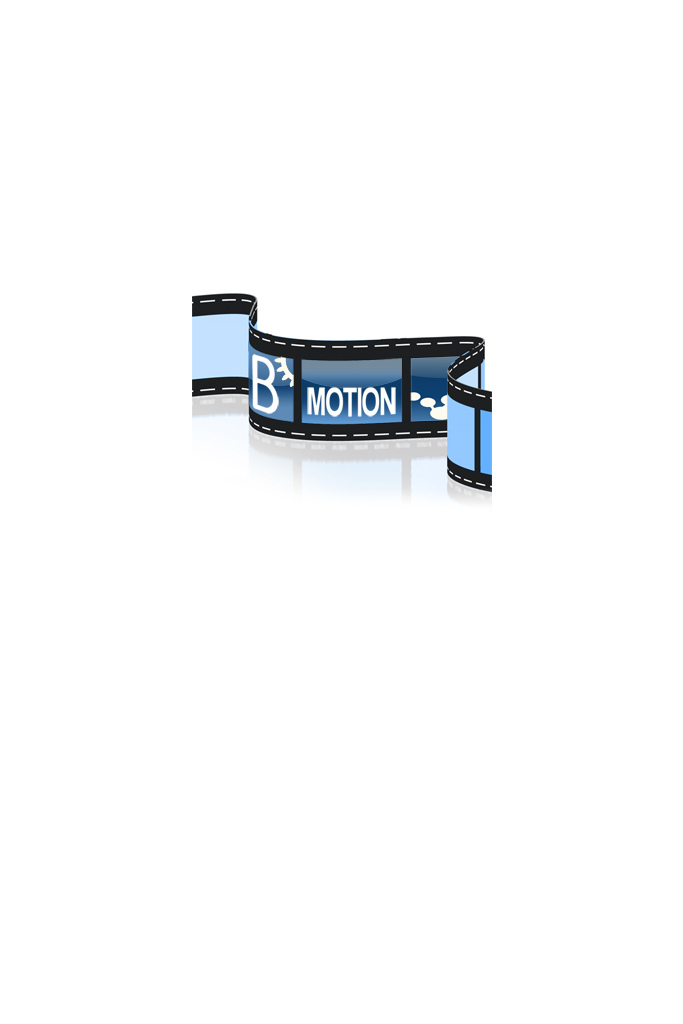
\includegraphics[width=\paperwidth,
keepaspectratio]{img/bms-handbook-bg.jpg}%
\vfill
}}}

\fi

%%% Local Variables: 
%%% mode: latex
%%% TeX-master: "rodin-doc"
%%% End: 
